\documentclass[border=6pt]{standalone}
\usepackage{tikz}
\definecolor{strandA}{HTML}{159A9C}
\definecolor{strandB}{HTML}{9B1B9E}
\begin{document}
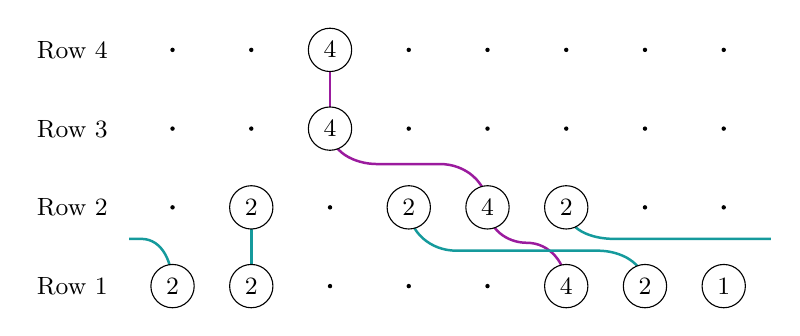
\begin{tikzpicture}[x=1cm,y=1cm,
  ball/.style={circle,draw,inner sep=0pt,minimum size=5.5mm,font=\small,fill=white},
  pt/.style={circle,fill=black,inner sep=0pt,minimum size=1.6pt},
  sA/.style={strandA,line width=0.9pt},
  sB/.style={strandB,line width=0.9pt}]
  % grid of positions
  \foreach \r in {1,...,4} {
    \node[font=\small,anchor=east] at (0.3,\r) {Row \r};
    \foreach \c in {1,...,8} \node[pt] at (\c,\r) {};
  }
  % pairings (drawn first, balls on top)
  \draw[sB] (3,4) -- (3,3);                                   % trivial pairing, new layer
  \draw[sB] (3,3) to[out=-90,in=180] (3.6,2.55) -- (4.4,2.55) to[out=0,in=90] (5,2);
  \draw[sB] (5,2) to[out=-90,in=180] (5.5,1.55) to[out=0,in=90] (6,1);
  \draw[sA] (2,2) -- (2,1);
  \draw[sA] (4,2) to[out=-90,in=180] (4.6,1.45) -- (6.4,1.45) to[out=0,in=90] (7,1);
  \draw[sA] (6,2) to[out=-90,in=180] (6.6,1.6) -- (8.6,1.6);
  \draw[sA] (0.45,1.6) -- (0.6,1.6) to[out=0,in=90] (1,1);
  % balls
  \node[ball] at (3,4) {4};
  \node[ball] at (3,3) {4};
  \foreach \c/\l in {2/2,4/2,5/4,6/2} \node[ball] at (\c,2) {\l};
  \foreach \c/\l in {1/2,2/2,6/4,7/2,8/1} \node[ball] at (\c,1) {\l};
\end{tikzpicture}
\end{document}
